% !TeX spellcheck = cs_CZ
\begin{mdframed}[style=mdexam]
\begin{example}\label{TEO:ex_DifOpamp01} 
  Uvažujme diferenciální zesilovač s ideální operačním zesilovačem typu VFA s naznačenými 
  uzly tak, jak je na obr. \ref{TEO:fig_MMUN_diff_opamp}. Napište rovnice MMUN.

   {\centering
    \captionsetup{type=figure}
    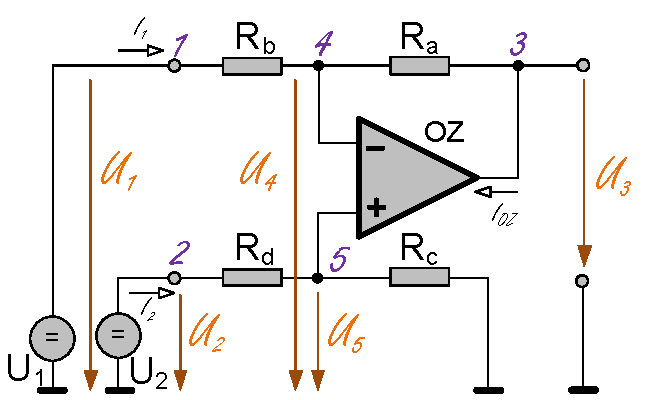
\includegraphics[width=0.7\linewidth]{MMUN_diff_OPAMP.pdf}
    \captionof{figure}{ Diferenciální zesilovač}
    \label{TEO:fig_MMUN_diff_opamp}
    \par}

    % using \usepackage{array} and command \newcolumntype{C}[1]{>{\centering}m{#1}}!
    {\centering
    \begin{tabular}{|C{0.6cm}|C{0.6cm}|C{0.6cm}|C{1.2cm}|C{0.6cm}|C{0.45cm}|C{0.45cm}|C{0.45cm}|}
        \multicolumn{1}{c}{$U_1$}  & \multicolumn{1}{c}{$U_2$}   & \multicolumn{1}{c}{$U_3$}  & 
        \multicolumn{1}{c}{$U_4$}  & \multicolumn{1}{c}{$U_5$}   & \multicolumn{1}{c}{$I_1$}  & 
        \multicolumn{1}{c}{$I_2$}  & \multicolumn{1}{c}{$I_{OZ}$}                      \\
        \hline
        $G_b$  &        &        & $-G_b$    &         & \(-1\) &        &             \\
        \hline
               & $G_d$  &        &           & $-G_d$  &        & \(-1\) &             \\
        \hline
               &        &  $G_a$ & $-G_a$    &         &        &        &             \\
        \hline 
        $-G_b$ &        & $-G_a$ & $G_a+G_b$ &         &        &        &             \\
        \hline
               & $-G_d$ &        & $G_c+G_d$ &         &        &        &             \\
        \hline
               &        &        &  \(-1\)   &  \(1\)  &        &        &             \\
        \hline
         1     &        &        &           &         &        &        &             \\
        \hline   
               & \(1\)  &        &           &         &        &        &             \\
        \hline    
    \end{tabular}
    \par}
\end{example}
\end{mdframed}